\documentclass{tudphygp_eng}
\usepackage{tudphymd,mhchem,lmodern,mathtools,mdwlist,multirow}

\versuch{Specific charge of an electron}{ER}
\author{G.~Oertel,R.~Schwierz}
\bearbeitet{A.~Otto, R.Mertzig}{}

\begin{document}
\maketitle

\section{Description}
  The specific charge $e/m$ of the electrons will be determined four different ways using a Thomson tube and a pair of coils in the Helmholtz configuration.
  \begin{enumerate}
    \item The electron beam will be steered with known acceleration potential $U_B$ and a $\vec B$-field of known strength. With $U_B$, $\vec B$, and the steering radius $R$,  $e/m$ will be determined.
    \item The electron beam will be guided through a defined point $(x,y)$ using an $\vec E$-field. The steering will be compensated by a magnetic field. With $\vec E$, $\vec B$, and the coordinates of the point, $e/m$ will be determined.
    \item The electron beam will be steered using a $\vec B$-field. The steering will be compensated by a $\vec E$-field. With $\vec E$, $\vec B$, and the geometry, $e/m$ will be determined.
    \item $\vec E$- and $\vec B$-field will be superimposed considering the known accelerator potential so that they compensate themselves. $e/m$ will be determined by $\vec E$, $\vec B$ and $U_B$.
  \end{enumerate}

\section{Basics}
\subsection{Deflection in the $\vec E$-field}
  An electron moves in an electrical field with the strength of $\vec E$. That electron experiences the force $\vec F$ and the acceleration $\vec a$.
  \begin{equation}
    \vec F = m\cdot\vec a = e\cdot\vec E
  \end{equation}
  The kinetic energy of the electron changes while passing a potential difference $U_B$.
  \begin{equation}
    \Delta E_K = e\cdot U_B
  \end{equation}
  Electrons created in a source ($E_{K0} = 0$) and accelerated have a velocity 
  $v$ after passing the potential difference $U_B$
  \begin{equation}
    e\cdot U_B = \frac{m}{2}\,v^2 \quad\text{resp.}\quad \frac{e}{m} = \frac{v^2}{2\cdot U_B}
    \label{for:E-Feld}
  \end{equation}
  The electron entering an $\vec E$-field opposite to the $y$-direction with a velocity of $\vec v = v_x\cdot \vec e_x$ 
  will be accelerated in the $y$-direction.
  \begin{equation}
    y=\frac{a_y}{2}\,t^2 = \frac{e\cdot E}{2\cdot m}\,t^2
  \end{equation}
  With $x = v_x\cdot t$, that leads to a trajectory according to the parabolic equation.
  \begin{equation}
    y=\frac{e\cdot E\cdot x^2}{2\cdot m\cdot v_x^2}
    \label{for:parabelgleichung}
  \end{equation}

\subsection{Deflection in the $\vec B$-field}
  An electron experiences the Lorentz-force in a magnetic field
  \begin{equation}
    \vec F = -e\cdot \vec v \times \vec B
  \end{equation}
  If an electron with the velocity $\vec v$ leaves the electron gun into a homogenous magnetic field perpendicular to the direction of movement, it experiences a force of constant strength. That force guides the electron in a circular trajectory with the radius $R$.
  This force is defined by:
  \begin{equation}
    F = \frac{m\cdot v^2}{R} = e\cdot v\cdot B \implies v = \frac{e}{m}\cdot B\cdot R
    \label{for:B-Feld}
  \end{equation}
  
\subsection{The field of the Helmholtz-coils}
  \parpic[]{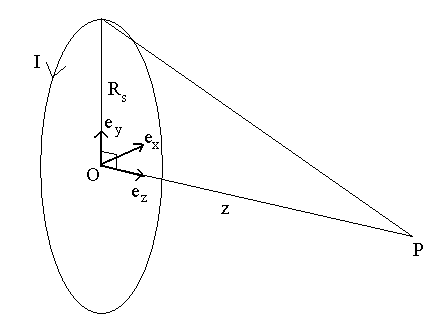
\includegraphics[width=0.40\textwidth]{helmholtz.png}}
  The Helmholtz-configuration is defined by two coils with the number of windings $n_1 = n_2$ and radius $R$, which are positioned to each other a distance $R$. A homogenous field will be created in the space between both coils. 
	According to Biot-Savart:
  \begin{equation}
    \vec B = \frac{\mu_0 I}{4\pi}\,\Int\frac{\diff\vec r\,^\prime \times \kla{\vec r-\vec r\,^\prime}}
    {\left|\vec r-\vec r\,^\prime\right|^3}
  \end{equation}
  $\vec r\,^\prime$ is the coordinate of the current leading conductor. For a circular coil perpendicular to the z-axis at the position $z = 0$, the equation for the B-field on the $z$-axis results as:
  \begin{equation}
    \vec B = \frac{\mu_0 I\cdot n}{2}\frac{R_s^2}{\sqrt{R_s^2+z^2}^{\,3}}\,\vec e_z
  \end{equation}
  Assuming two coils at $z=-R_s/2$ and $z=+R_s/2$, each with $n$ windings leading the current in the same direction, the equation describing the B-field on the $z$-axis is:
  \begin{equation}
    \vec B = \frac{\mu_0 I\cdot n}{2}\brk{\frac{R_s^2}{\sqrt{R_s^2+\kla{z-\frac{R_s}{2}}^2}^{\,3}}+
    \frac{R_s^2}{\sqrt{R_s^2+\kla{z+\frac{R_s}{2}}^2}^{\,3}}}\,\vec e_z
  \end{equation}
  The series expansion at $z=0$ leads to
  \begin{equation}
    \vec B(z) = \frac{\mu_0 I\cdot n}{R\cdot\sqrt{\kla{\frac{5}{4}}^3}}\cdot\kla{1-\frac{144}{125}\frac{z^4}{R_s^4}+\dots}
  \end{equation}
  meaning a very homogenous field with a deviation less than \SI{1}{\%} up to $z = \num{0.3}\cdot R_s$ .

\section{Experiments}
  \begin{figure}[h]
    \centering
    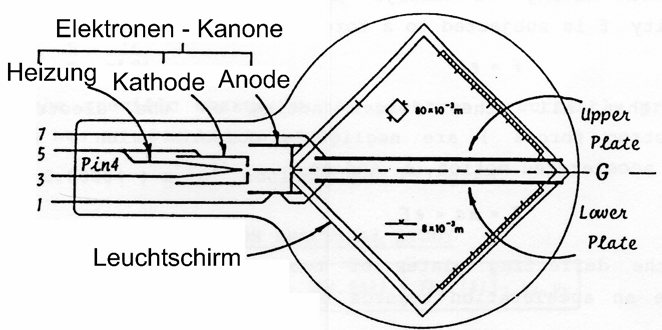
\includegraphics[width=0.8\textwidth]{thomsonroehre.png}
    \caption{Sketch of the Thomson tube}
  \end{figure}
  The Thomson tube is used to create a visible electron beam. Here electric and magnetic fields can be perpendicularly superimposed to each other. Both fields are able to steer the beam. The specific charge of the electron can be determined by solving the equations of motion.
  
  Connect the Thomson tube according to the following sketch:
  \begin{figure}[h]
    \centering
    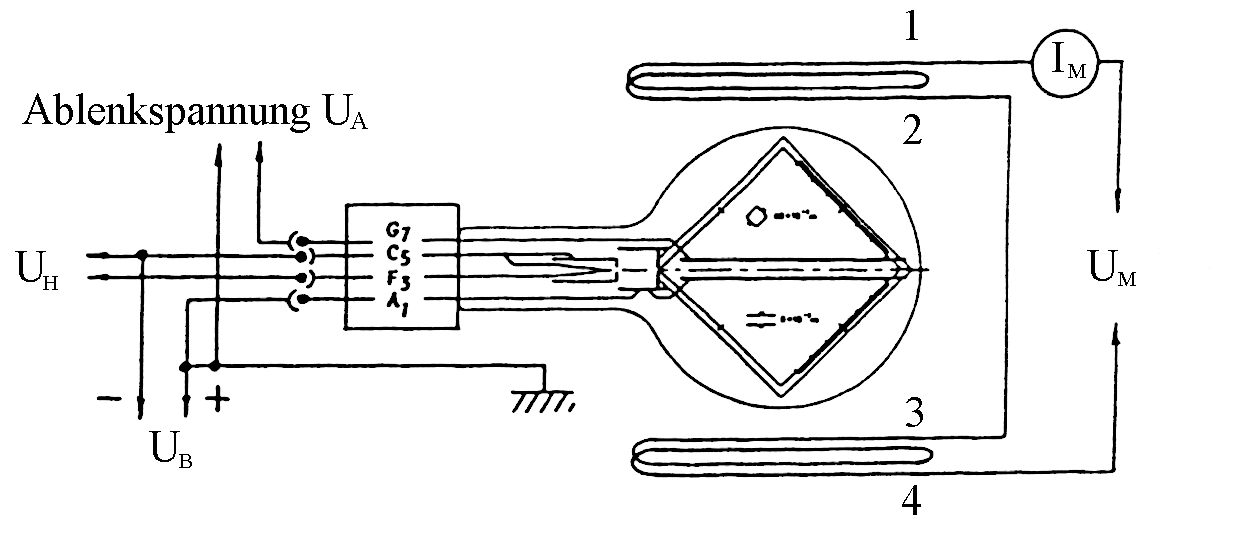
\includegraphics[width=0.8\textwidth]{schaltskizze.png}
    \caption{Sketch of the connections}
  \end{figure}
  
  \parpic[]{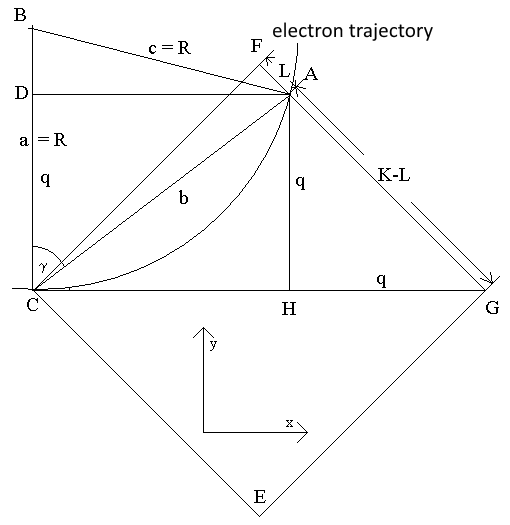
\includegraphics[width=0.30\textwidth]{elektronenbahn.png}}
  The anode $A_1$ has to be grounded and a negative voltage has to be applied at the cathode $C_5$. The trajectory  
  $R$ can be determined by the steering $L$:
  
  The electron beam leaves the electron gun at C and moves toward the $x$-direction while getting steered into the $y$-direction. 
  The circular trajectory has the radius $R$. 
  
  In the tube is a square positioned on one edge, with the vertices: 
  C, E, F, G; in addition is the edge length $K = \SI{80}{mm}$ known, the length $L = \abs{\mathrm{FA}}$ 
  is readable.

  For the radius $R$ follows:\picskip{0}
  \begin{flalign*}
    &\triangle\text{ A,B,C: } c^2 = a^2+b^2-2ab\cdot\cos\gamma \xRightarrow{a=c=R} \cos\gamma=\frac{b}{2a} &\\
    &\triangle\text{ A,C,D: } \cos\gamma = \frac{q}{b} = \frac{b}{2a} \implies R=a=\frac{b^2}{2q} &\\
    &\triangle\text{ A,C,F: } b^2 = K^2+L^2 &\\
    &\triangle\text{ A,G,H: } (K-L)^2 = q^2+q^2 \implies q=\sqrt\frac{(K-L)^2}{2} &\\
    &\implies R^2 = \frac{1}{2}\,\kla{\frac{K^2+L^2}{K-L}}^2 \text{ and if} L=0 \implies R = \frac{1}{\sqrt{2}}\,K &
  \end{flalign*}

\subsection{Experiment 1: Classic Thomson-experiment}
  For evaluating $e/m$ (see eq. \eqref{for:E-Feld}) the electron velocity $v$ after passing the accelerator potential $U_B$ will be determined by measuring the trajectory $R$ of the electrons in a homogenous magnetic field (see eq. 
  \eqref{for:B-Feld}):
  \begin{equation}
    \frac{e}{m} = \frac{2U_B}{B^2\cdot R^2}
  \end{equation}
  \textbf{Execution:}
  \begin{enumerate}
    \item Ground the upper steering plate.
    \item Adjust the accelerator potential to $U_B=\SI{455}{V}$ .
    \item Correctly connect the Helmholtz coils and adjust the current for the coils so that the beam passes an easily observable point.
    \item Vary coil current and accelerator potential while keeping the beam passing this point. Record the values $U_B$, $I_M$ , plot $I_M^2$ dependent on $U_B$, and determine the slope.\\
    \begin{minipage}{0.45\textwidth}
    \centering
    \begin{tabular}{|c|c|c|c|}\hline
      $L/\SI{}{mm}$ & $U_B/\SI{}{V}$ & \hspace{10pt}$I_M/\SI{}{A}$\hspace{10pt} & \hspace{10pt}$I_M^2/\SI{}{A^2}$\hspace{10pt} \\\hline
      $0/40$        &     2000       &                &                   \\
      $0/40$        &     2500       &                &                   \\
      $0/40$        &     3000       &                &                   \\
      $0/40$        &     3500       &                &                   \\
      $0/40$        &     4000       &                &                   \\
      $0/40$        &     4500       &                &                   \\\hline
    \end{tabular}
    \end{minipage}
    \hfill
    \begin{minipage}{0.45\textwidth}
    \centering
    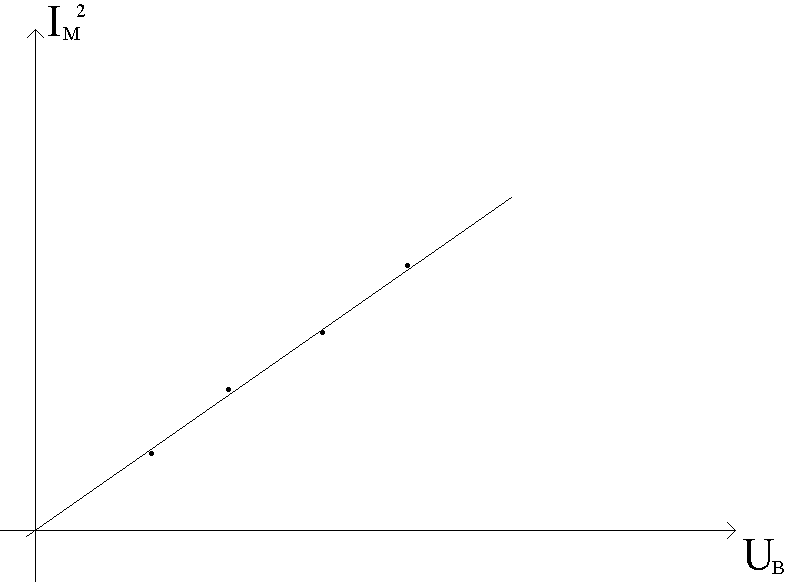
\includegraphics[width=\textwidth]{diagramm.png}
    \end{minipage}
    \item Determine $e/m$ from those values.
    \item What is the value of $v$ at $U_B=\SI{4.0}{kV}$? What is the strength of $\abs{\vec B}$ at $R=\frac{K}{\sqrt{2}}$ and $U_B=\SI{4.0}{kV}$?
  \end{enumerate}
  
\subsection{Experiment 2: The field compensation experiment}
  The direction of motion of the electrons always changes under influence of the Lorentz-force. 
	If the Lorentz-force is compensated by the electric field, the direction of motion and the velocity of the electrons remain constant.  
  \begin{equation}
    e\cdot E = e\cdot v_x\cdot B \implies v_x=\frac{E}{B}
    \label{for:v_x}
  \end{equation}
  leads to $v_x$ in \eqref{for:parabelgleichung}
  \begin{equation}
    y(x) = x^2\,\frac{e\cdot B^2}{2mE},
  \end{equation}
  which is used for calculating $e/m$ .\\
	$y$- and $x$ are defined as the coordinates of the electron beam under the influence of the steering $\vec E$-field. Soldered pins at $x=\SI{47}{mm}$ and $d/2=y=\pm\SI{4}{mm}$, where the electron beam is steered only by the $\vec E$-field, will be used for an exact steering of the electron beam through a point. 
  $E=U_A/d$ leads to:
  \begin{equation}
    \frac{e}{m} = \frac{U_A}{x^2\cdot B^2}
  \end{equation}
  \begin{figure}
    \centering
    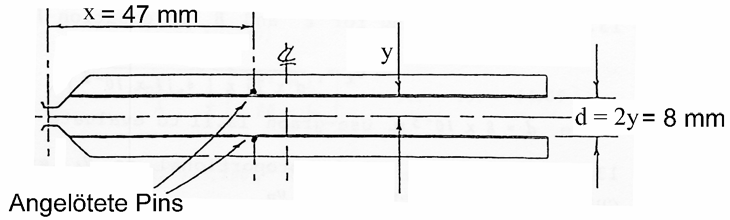
\includegraphics[width=0.8\textwidth]{feldausgleich.png}
    \caption{Zur Definition von $x$, $y$ und $d$}
  \end{figure}
  \textbf{Execution:}
  \begin{enumerate}
    \item Adjust the accelerator potential $U_B$ to approx. \SI{4}{kV} and $U_A$ to \SI{150}{V} . The beam will be steered close to one of the pins.
    \item Adjust $U_B$ to that value, where the beam is blocked by a pin.
    \suspend{enumerate}
      These adjustments shouldn't change until finalizing the measurement of $I_M$.
    \resume{enumerate}
    \item Adjust the magnetic field again so that the beam is forced to pass G. Record $U_A$ and $I_M$.
    \item Vary $U_A$ in steps of \SI{50}{V} and repeat 2. and 3., record $U_A$ and $I_M$. Plot $I_M^2$ 
    dependent on $U_A$ and determine the slope.\\[1em]
    \begin{tabular}{|c|c|c|}\hline
      $U_A/\SI{}{V}$ & \hspace{10pt}$I_M/\SI{}{A}$\hspace{10pt} & \hspace{10pt}$I_M^2/\SI{}{A^2}$\hspace{10pt} \\\hline
      150 & &\\
      200 & &\\
      250 & &\\
      300 & &\\
      350 & &\\\hline
    \end{tabular}
    \item Determine $e/m$ from the slope.
  \end{enumerate}

\subsection{Experiment 3}
  Using the results gained in experiment 2 (equations \eqref{for:B-Feld}, \eqref{for:v_x}), considering $E=U_A/d$ leads to:
  \begin{equation}
    \frac{e}{m} = \frac{U_A}{B^2\cdot R\cdot d}
  \end{equation}
  $R$ is defined as the radius of the trajectories of the electrons in the $\vec B$-field without the influence of the $\vec E$-field. This expression can be rewritten as:
  \begin{equation}
    I_M^2 = k\,\frac{U_A}{R}
  \end{equation}
  \textbf{Execution:}
  \begin{enumerate}
    \item Adjust $U_B \approx \SI{2.5}{kV}$
    \item Adjust $U_A = \SI{100}{V}$ and compensate the bending of the beam by adjusting the coil current until the beam passes point G.
    \item Ground the steering plate again and record the value of $L$.
    \item Repeat those steps for different $U_A$ and record $U_A$, $I_M$, $L$.\\[1em]
    \begin{tabular}{|c|c|c|c|c|}\hline
      $U_A/\SI{}{V}$ & \hspace{10pt}$I_M/\SI{}{A}$\hspace{10pt} & \hspace{10pt}$I_M^2/\SI{}{A^2}$\hspace{10pt} & \hspace{10pt}$L/\SI{}{mm}$\hspace{10pt} & \hspace{10pt}$R/\SI{}{mm}$\hspace{10pt} \\\hline
      100 & & & &\\
      150 & & & &\\
      200 & & & &\\\hline
    \end{tabular}
    \item Evaluate $e/m$ from the measured values.
  \end{enumerate}
  
\subsection{Experiment 4}
  Using the knowledge gained from experiment 2 (equations \eqref{for:E-Feld}, \eqref{for:v_x}), and using $E=U_A/d$, leads to:
  \begin{equation}
    \frac{e}{m} = \frac{1}{2\cdot U_B}\,\kla{\frac{U_A}{B\cdot d}}^2 \quad\text{also:}\quad I_M^2 = k\,\frac{U_A^2}{U_B}
  \end{equation}
  \textbf{Execution:}
  \begin{enumerate}
    \item Adjust the accelerator potential to $U_B = \SI{4}{kV}$ .
    \item Adjust the steering potential to $U_A = \SI{100}{V}$ .
    \item Adjust the magnetic field until the beam passes point G again.
    \item Record potentials and coil current, vary $I_M$ at constant accelerator potential $U_A$, plot $I_M$ dependent on $U_A$, and determine the slope of two accelerator potentials.\\[1em]
    \begin{tabular}{|c|c|c|}\hline
      $U_B/\SI{}{V}$ & $U_A/\SI{}{V}$ & \hspace{10pt}$I_M/\SI{}{A}$\hspace{10pt} \\\hline
      \multirow{5}{*}{4000} & 100 &\\
       & 150 &\\
       & 200 &\\
       & 250 &\\
       & 300 &\\\hline
    \end{tabular}
    \item Determine $e/m$ from the slopes.
  \end{enumerate}
  
\frage{Which other experimental approaches for determining the specific charge do you know?}
\frage{Which approaches for determining the charge of the electron are available?}
\frage{How are the trajectories of the electrons guided if $\vec v$ is not perpendicular to $\vec B$ ?}
\frage{Discuss in detail the influence of the magnetic field of the earth. How can the strength be guessed or reduced?}
\frage{The homogenous magnetic field is generated by two coils which are serially connected. How can one check if they are connected correctly?}
\frage{Outline the circuit for switching over the polarity of the current which flows through the pair of Helmholtz coils.}

\end{document}
